%%%%%%%%%%%%%%%%%%%%%%%%%%%%%%%%%%%%%%%%%%%%%%%%%%%%%%%%%%%%%%%%%%%%%%%%%%%%%%%%
\chapter{РАЗРАБОТКА}
%%%%%%%%%%%%%%%%%%%%%%%%%%%%%%%%%%%%%%%%%%%%%%%%%%%%%%%%%%%%%%%%%%%%%%%%%%%%%%%%

\section{Разработка подмодулей, не зависящих от web-приложения}

Разрабатываемый модуль должен быть легко подключаем к web-приложению. Поэтому было решено сделать файл softPhone.js, который подключает модуль softPhone.html AJAX-запросом. SoftPhone.html включает в себя разметку кнопок плавающего окна, подключает аудио-файлы звонка и гудков, а также подключает остальные подмодули:
\begin{itemize}
\item SIPml-api.js - подмодуль библиотеки sipML5.
\item softPhoneCore.js - подмодуль, отвечающий за аутентификацию клиента на сервере SIP-телефонии, и осуществление звонков. Также в нём отслеживаются события звонка (CallEvents).
\item softPhonePopupUI.js - подмодуль обработки плавающего окна при перетаскивании мышью.
\item softPhone.css - подмодуль разметки плавающего окна.
\item softPhone\_"web-app".js\footnote{здесь "web-app" означает название web-приложения, к которому будет подключатся модуль} - подмодуль, в котором размещается функция getSipAccount() для конкретного web-приложения.
\item softPhone\_"web-app".php - подмодуль, отправляющий sipAccountInfo клиенту.
\end{itemize}

Основные функции подмодуля softPhoneCore.js:
\begin{itemize}
\item createSipStack() - инициирует конфигурацию SIP-соединения, основываясь на информации полученной getSipAccount().
\item register() - аутентификация SIP-клиента на сервере.
\item unregister() - деаутентификация SIP-клиента на сервере, выполняется при закрытии web-страницы, если не было сделанно вручную.
\item onSipEventStack(e) - обработчик событий управляющей созданием или завершением SIP-сессий. Сессия аутентификации создаётся после аутентификации, а сессия звонка создаётся при входящем или исходящем звонке. Такие события поступают от сервера.
\item onSipEventSession(e) - обработчик событий SIP-сессий. Обрабатываются события ответа на звонок и сброса. Такие события поступают от собеседника.
\item call() - обработчик кнопки вызова.
\item hangup() - обработчик кнопки сброса.
\item finalState(action) - функция конечного автомата, управляющего состоянием SIP-клиента (см. рисунок \ref{image:FinalState}). В состоянии calling мы слышим гудки, а в состоянии incoming мы слышим рингтон. Также здесь происходит включение и выключение кнопок Call и HangUp.
\item startRingTone(), stopRingTone(), startRingbackTone() и stopRingbackTone() - функции воспроизведения и останова воспроизведения рингтона и гудков.
\end{itemize}

\begin{figure}[h!]
\center{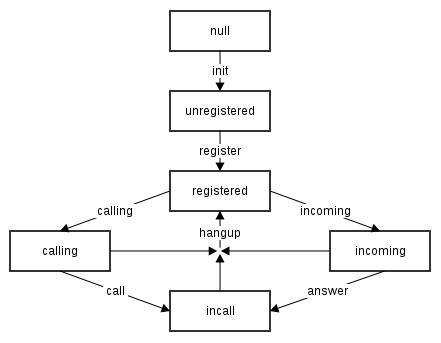
\includegraphics[width=0.75\linewidth]{FinalState}}
\caption{Конечный автомат, управляющий состоянием SIP-клиента}
\label{image:FinalState}
\end{figure}

Основные функции подмодуля softPhonePopupUI.js:
\begin{itemize}
\item show\_hide\_popup() - функция отображения и скрытия всплывающего окна.
\item mouseDown(e), mouseUp() и popupMove(e) - функции перетаскивания всплывающего окна.
\end{itemize}

\section{Разработка подмодулей, зависящих от web-приложения, на примере SalesPlatform vtiger CRM 6.4}

Модуль софт-фона будет очень полезен для CRM-систем. Операторам компаний будет намного удобнее осуществлять звонки из CRM-системы прямо в браузере и создавать комментарии к звонкам. В CRM-системе SalesPlatform vtiger CRM 6.4 имеется модуль PBXManager, который осуществляет звонки при помощи стороннего настольного или мобильного приложения, или же аппаратного SIP-телефона. При осуществлении вызова через CRM-систему, система сообщает серверу SIP-телефонии, что происходит вызов, тогда стороннее приложение или аппаратный SIP-телефон начинает звонить. Во время звонка в CRM-системе создаётся карточка звонка.

Подмодули softPhone\_vtiger.js и softPhone\_vtiger.php были разработаны для CRM-системы SalesPlatform vtiger CRM 6.4. Подмодуль softPhone\_vtiger.js содержит функцию getSipAccount(), которая осуществляет AJAX-запрос данных о SIP-аккаунте (ip-адрес и порт сервера телефонии, SIP-номер и пароль для текущего пользователя CRM-системы). А подмодуль softPhone\_vtiger.php отвечает на этот запрос. Для этого он анализирует данные о сессии пользователя, и, обращаясь к другим модулям CRM-системы, получает информацию о SIP-аккаунте текущего пользователя.

Так же подмодуль softPhone\_vtiger.js должен генерировать и отправлять данные о состоянии звонка, а softPhone\_vtiger.php должен их получать и генерировать карточки звонков, которые заполняются операторами.

Однако эти задачи очень трудоёмки, так как исходный код данной CRM-системы очень большой, и поэтому выполнены не были. Получение информации о SIP-аккаунте было прописано только для одного пользователя. То есть любой пользователь, кто использует разработанный нами софт-фон, авторизуется за одного и того же пользователя на SIP-сервере. Так же не было реализовано создание карточек звонков в CRM-системе.

В функцию click-to-call модуля PBXManager было добавленно несколько строк кода, заполняющих поле набираемого номера в нашем модуле. То есть осуществив patch PBXManager, легко можно добавить click-to-call в разрабатываемый модуль.